\section*{Mise en situation}
\ifprof
\else
\fi

Le projet WHING a pour objet d'imaginer et de réaliser et proposer aux utilisateurs un fauteuil verticaliseur à déplacement motorisé de nouvelle génération avec, comme objectifs associés : 
\begin{itemize}
\item d'intégrer de nouvelles technologies; 
\item de mieux prendre en compte les besoins spécifiques des utilisateurs, 
\item d'utiliser une conception modulaire. 
\end{itemize}

Le fauteuil est équipé d'une base roulante à six roues indépendantes. Les roues centrales motrices autorisent un faible moyen de giration. La base roulante, forte de ses 6 roues indépendantes et amorties assure la stabilité et motricité du fauteuil, quel que soit le profil du terrain rencontré. 


\begin{center}
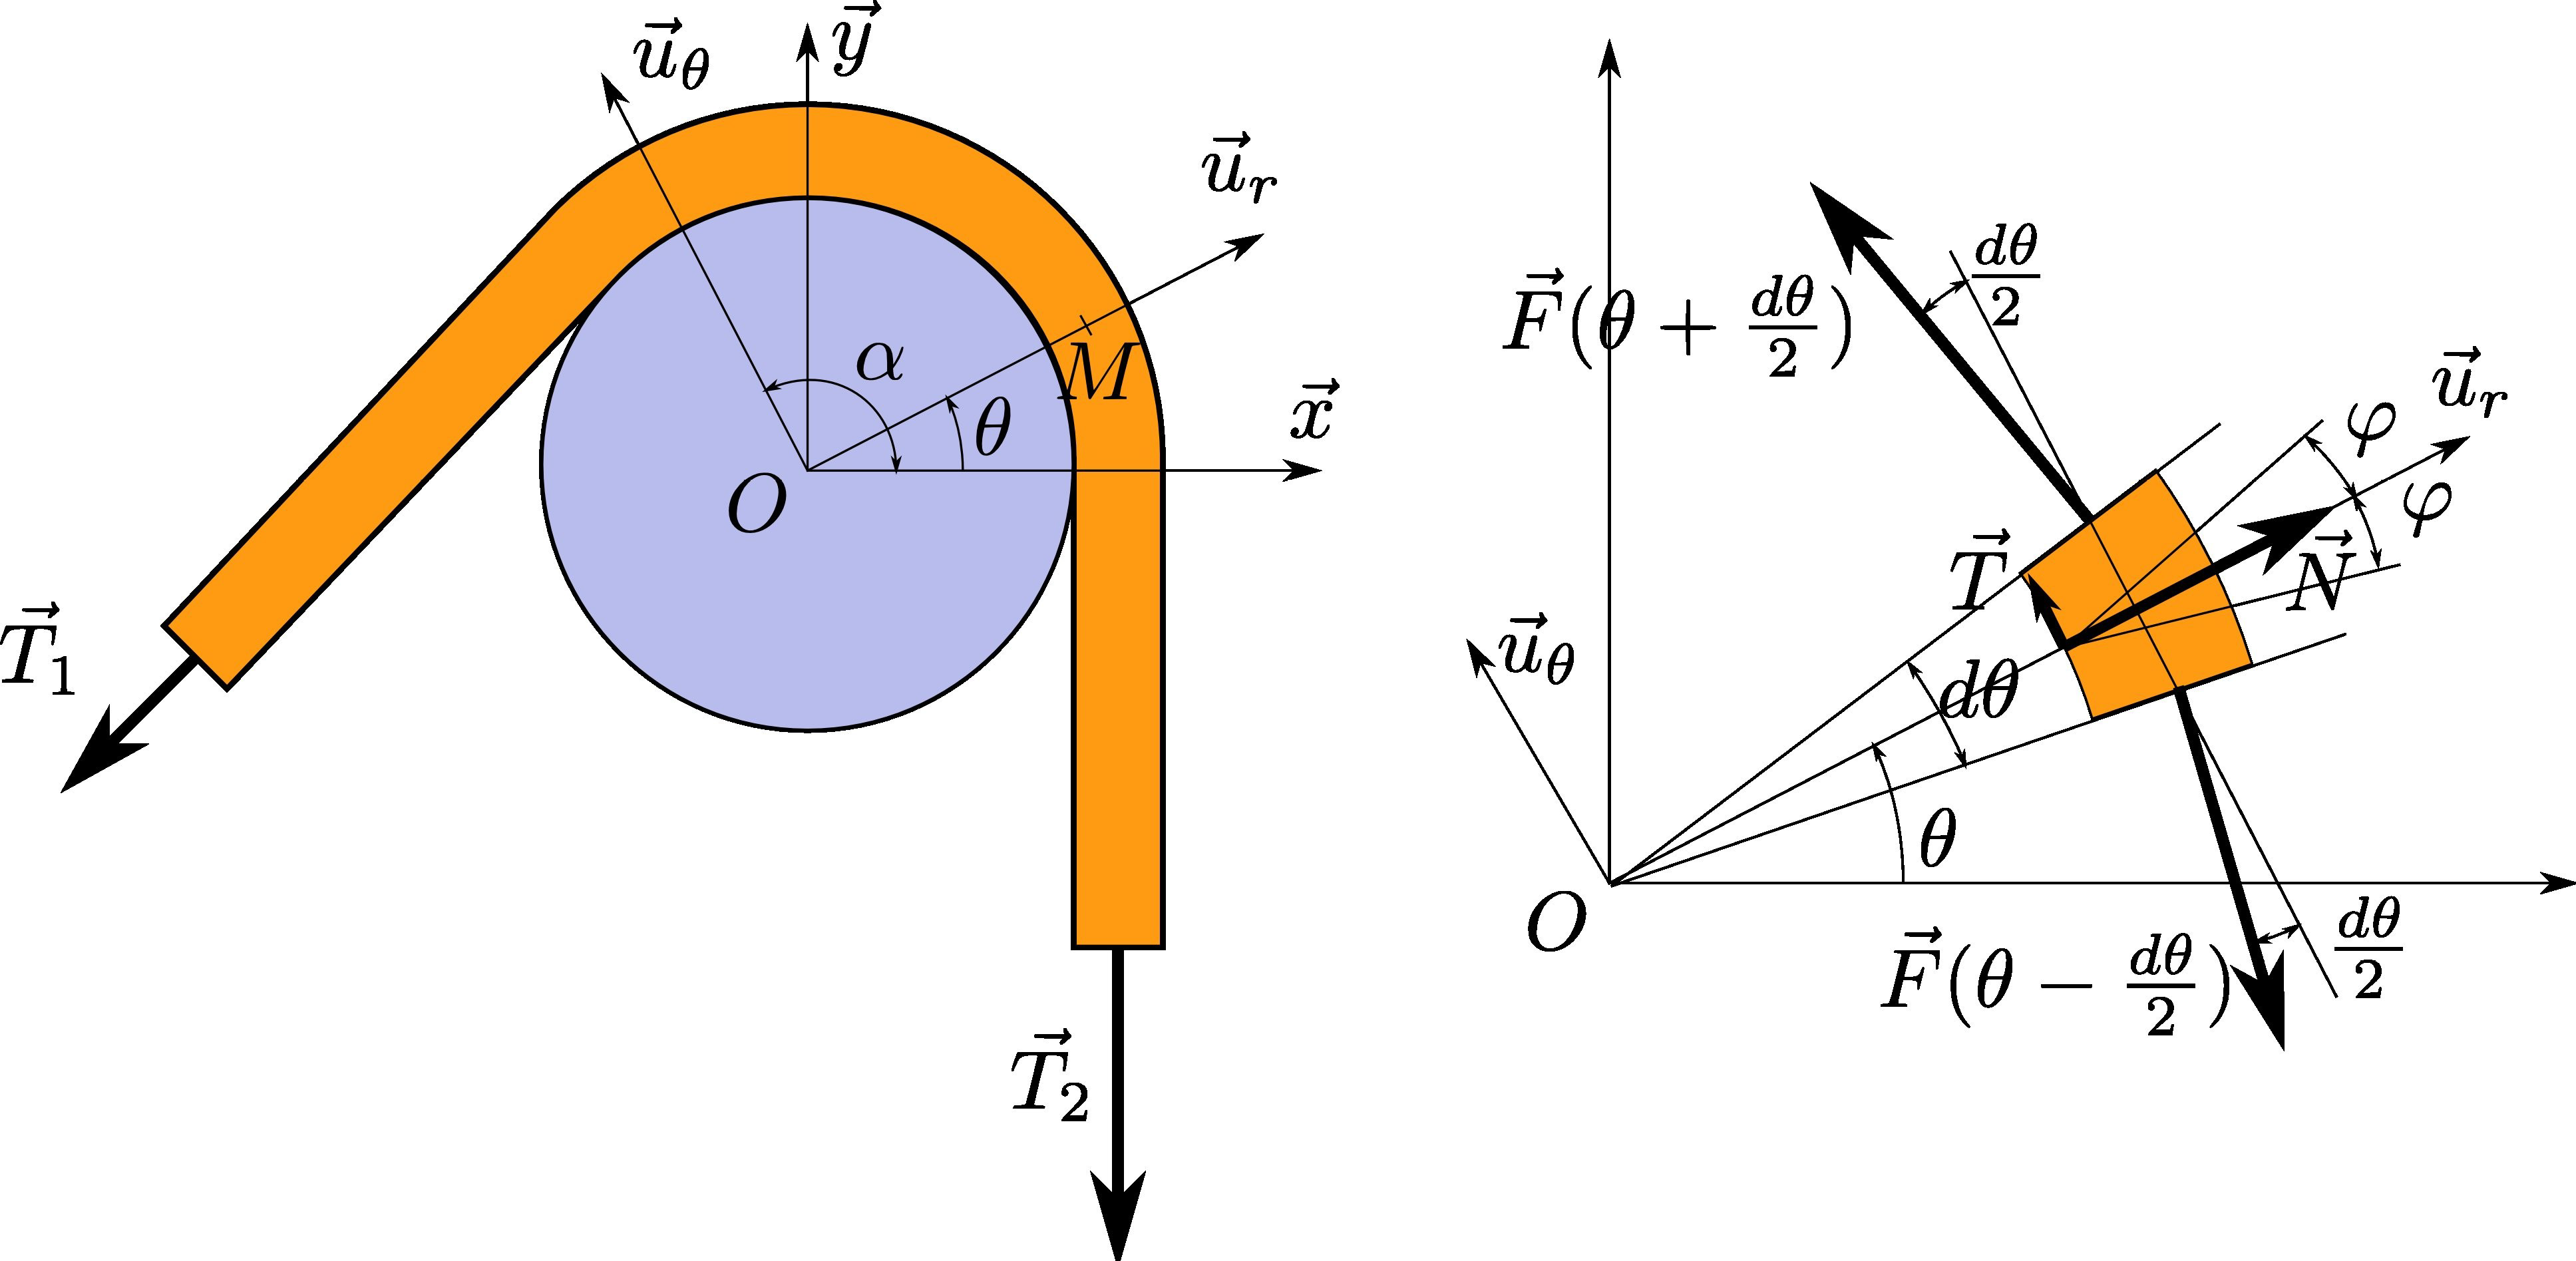
\includegraphics[width=.7\linewidth]{fig_01}
%\textit{}
\end{center}




\begin{obj} 
%Vérifier que les groupes motoréducteurs des roues motrices permettent le démarrage du
%WHING sur une pente de 15\degres.

L'exigence Id = <<~1.4.5~>> indique que le fauteuil doit être capable de gravir une pente pour
monter dans un véhicule de transport. La pente maximale est de 15\degres. Les caractéristiques du moteur-roue
sont données ci-dessous.
\end{obj}


\begin{center}
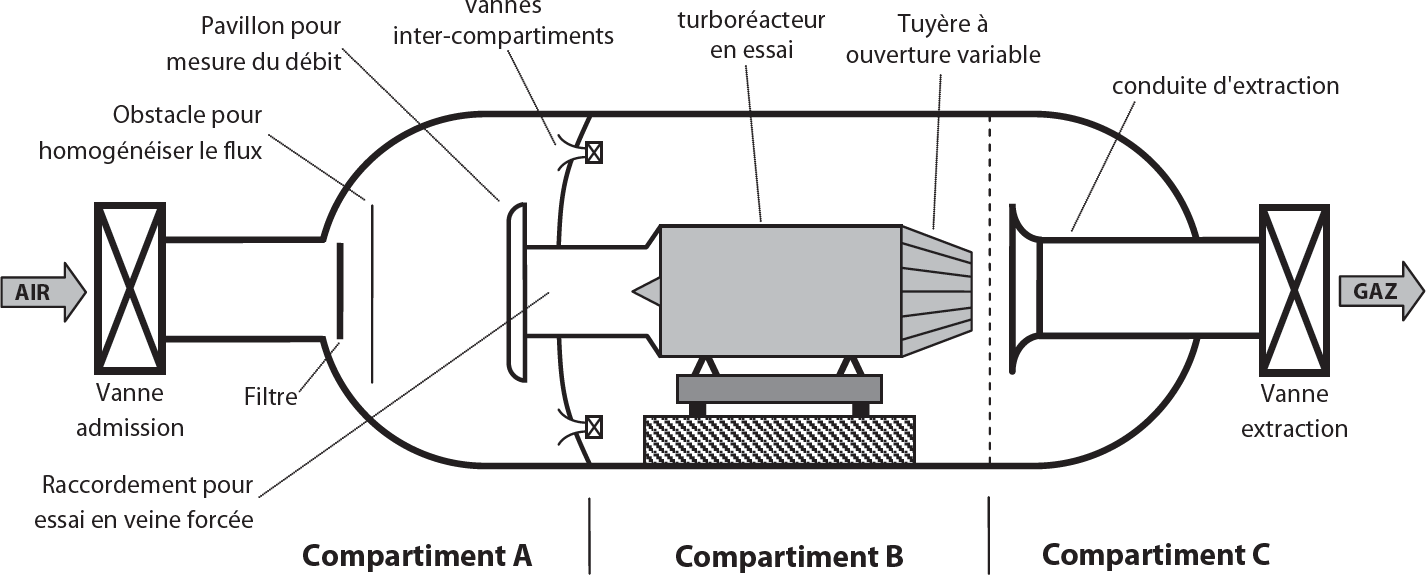
\includegraphics[width=.5\linewidth]{fig_02}
%\textit{}
\end{center}

Pour valider cette exigence, le cadre de l'étude est le suivant.
Les hypothèses d'étude sont :
\begin{itemize}
\item le référentiel $\rep{0}\repere{O}{x_0}{y_0}{z_0}$ lié au sol est supposé galiléen;
\item le WHING se déplace en ligne droite dans une phase de montée, le problème est considéré comme un problème plan. Les effets dynamiques sont négligés car la vitesse de déplacement du
fauteuil est faible;
\item le référentiel $\rep{1}\repere{O}{x_1}{y_1}{z_1}$ est lié au WHING avec $\vect{x_0}=\vect{x_1}$;
\item $\vect{P}=-mg\vect{z_0}$ est l'action de la pesanteur et $G$ le centre de gravité de l'ensemble \{fauteuil +
PMR\};
\item le modèle adopté est équivalent à un seul moteur fournissant un couple $C_m$ avec l'action de la
pesanteur ramenée au centre de gravité égale à $\dfrac{P}{2}$;
\item le contact des roues avec le sol se fait avec frottement, on note $f$ le facteur de frottement de valeur 0,45 ;
\item la résistance au roulement modélise la déformation du pneumatique.
\end{itemize}

La résistance au roulement illustrée à la figure suivante, se traduit par un décalage du point
d'application de l'action mécanique de contact vers l'avant du fauteuil (dans le sens de l'avancement). La résultante des forces passe en un point $A$ à une distance $\delta$ de l'axe de rotation.
Cette distance est par définition le coefficient de résistance au roulement.


\begin{center}
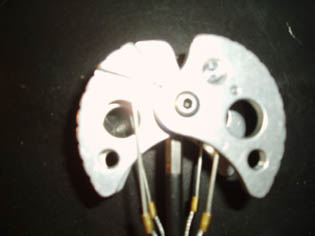
\includegraphics[width=.5\linewidth]{fig_03}
%\textit{}
\end{center}


La figure suivante donne le paramétrage de l'étude en phase de montée d'une pente et les dimensions du WHING. Les points $A_S$, $B_S$ et $C_S$  correspondent aux points d'application des actions mécaniques du sol sur les roues avant, motrices et arrière du fauteuil.


\begin{center}
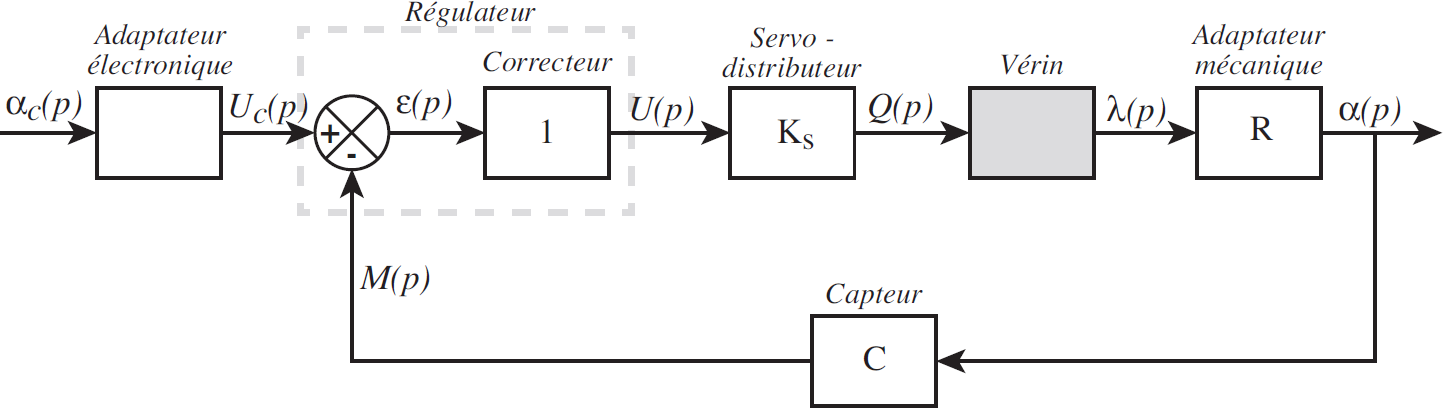
\includegraphics[width=\linewidth]{fig_04}
%\textit{}
\end{center}

\subsection*{Travail demandé}

\question{
Porter sur la figure précédente :
\begin{itemize}
\item l'action de la pesanteur ;
\item les actions de contact du sol sur les roues. Pour un point $A$, la composante normale sera notée $\vect{N_A}$ et la composante tangentielle $\vect{T_A}$. Le sens d'une composante tangentielle est différent si la roue
est motrice ou folle ;
\item le couple $\vect{C_{\text{red}}}$, couple à la sortie du réducteur du moteur-roue.
\end{itemize}}
\ifprof
\begin{corrige}
\end{corrige}
\else
\fi


\question{Appliquer le principe fondamental de la statique à l'ensemble WHING + PMR isolé et écrire les 3 équations dans la base $\rep{1}$ en fonction des données littérales. L'équation de moment sera exprimée
au point $B_S$.}
\ifprof
\begin{corrige}
\end{corrige}
\else
\fi



\question{Isoler la roue arrière puis la roue avant et déterminer une équation issue du principe fondamental de statique donnant la composante normale de l'action du sol sur la roue, en fonction des paramètres géométriques et de la composante tangentielle.}
\ifprof
\begin{corrige}
\end{corrige}
\else
\fi



\question{Isoler la roue motrice et déterminer une équation issue du PFS donnant $\vect{C_{\text{red}}}$ en fonction des données géométriques, de $\vect{N_{BS}}$ et $\vect{T_{BS}}$.}
\ifprof
\begin{corrige}
\end{corrige}
\else
\fi

En supposant que le contact du sol sur la roue motrice se fait à la limite du glissement, on obtient un système de 7 équations à 7 inconnues. 

La résolution de ce système donne les résultats suivants : $\vect{N_{BS}}\cdot \vect{z_1}=\SI{1140}{N}$ et $\vect{T_{BS}}\cdot \vect{y_1}=\SI{-350}{N}$.



\question{Justifier que la composante $\vect{T_{BS}}\cdot \vect{y_1}$ est négative. À partir des valeurs de $||\vect{T_{BS}}||$ et $||\vect{T_{BS}}||$, déterminer la valeur de $||\vect{C_m}||$ et conclure vis-à-vis des exigences du cahier des charges.}
\ifprof
\begin{corrige}
\end{corrige}
\else
\fi


%
%\question{}
%\ifprof
%\begin{corrige}
%\end{corrige}
%\else
%\fi

%
%
%\ifnormal
%\vspace{.5cm}
%
%\noindent \textbf{Éléments de corrigé}
%\vspace{-.5cm}
%\begin{multicols}{2}
%\begin{enumerate}
%\item \SI{1,26}{rad.s^{-1}}.
%\item \SI{1292}{tr.min^{-1}}.
%\item Oui.
%\item $I$.
%\item  $\torseurl{ F_B\vect{x_{2}}}{\vect{0}}{B}$.
%\item $ F_B    = \dfrac{mgx_G}{L_2  \sin  \left(\alpha_{12}-\alpha_2\right)} $.
%\item $C_{\text{red}}-RF_B \sin \left( \alpha_3 - \alpha_2\right) = 0$.
%\item \SI{252}{Nm}.
%\item \SI{2,34}{Nm}.
%\end{enumerate}
%%\item Angle d'ouverture: $67,5\degres$.
%%\item $L^2 =\left(-a + c\cos\theta \right)^2 + \left(b + c\sin\theta \right)^2  $.
%%\item Course de \SI{13,2}{cm}.
%%\item $   F_v = \dfrac{\lambda Mg\cos \theta}{c\sin \left( \alpha - \theta\right)} $ ($F_v/2$).
%%\item $k=\SI{1667}{N.m^{-1}}$, écrasement de $\SI{300}{mm}$.
%%\item .
%%\item $\Delta F = \pm \SI{443}{N}$.
%%\item $I_{\text{max}} = \SI{3,95}{A}$.
%%\end{enumerate}
%\end{multicols}
%\else
%\fi
%\fi
%
%\normalsize



\ifprof

\begin{center}
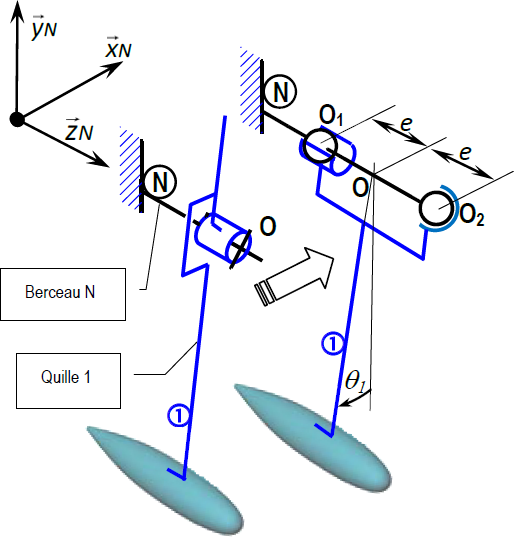
\includegraphics[width=.8\linewidth]{fig_05}
%\textit{}
\end{center}

\begin{center}
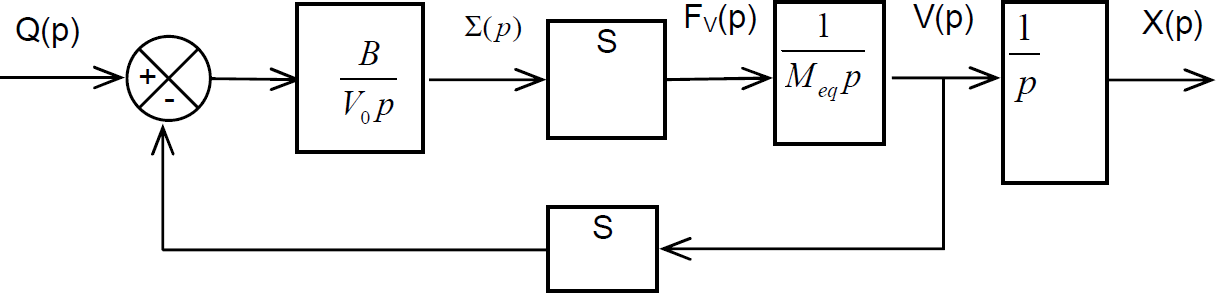
\includegraphics[width=\linewidth]{cor_01}
%\textit{}
\end{center}

\begin{center}
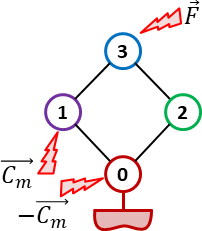
\includegraphics[width=\linewidth]{cor_02}
%\textit{}

\end{center}

\else
\fi